%%%%%%%%%%%%%%%%%%%%%%%%%%%%%%%%%%%%%%%%%%%%%%%%%%%%%%%%%%%%%%%%%%%%%%%
%% $Id: report.tex,v 1.5 2005/02/09 21:06:42 lindstrm Exp $
%%%%%%%%%%%%%%%%%%%%%%%%%%%%%%%%%%%%%%%%%%%%%%%%%%%%%%%%%%%%%%%%%%%%%%%
%% costhesis usage example
%% modified and added to by GQMJr
%%%%%%%%%%%%%%%%%%%%%%%%%%%%%%%%%%%%%%%%%%%%%%%%%%%%%%%%%%%%%%%%%%%%%%%
%
% The costhesis package accepts the following options
%
%   Document types:
%     msc               - Master Thesis
%     bsc		- Kandidate Thesis
%
%   Layout options:
%
%   Other options:
%     blank             - Removes pagenumbers and headers from empty pages
%     blankmsg          - Prints a message of intent on empty pages
%     scheader          - Typeset headers in SMALL CAPS shape (default)
%     slheader          - Typeset headers in slanted shape 
%
%
%
%

\documentclass[12pt,a4paper,twoside,openright]{book}
%%\documentclass[12pt,a4paper,twoside,openright]{memoir}

\usepackage[msc,blankmsg]{costhesis}
%\usepackage[T1]{fontenc}
%%\usepackage{pslatex}
\renewcommand{\rmdefault}{ptm} 
\usepackage{mathptmx}
\usepackage[scaled=.90]{helvet}
\usepackage{courier}
%
\usepackage{bookmark}

%%----------------------------------------------------------------------------
%%   pcap2tex stuff
%%----------------------------------------------------------------------------
 \usepackage[dvipsnames*,svgnames]{xcolor} %% For extended colors
 \usepackage{tikz}
 \usetikzlibrary{arrows,decorations.pathmorphing,backgrounds,fit,positioning,calc,shapes}
 \usepackage{pgfmath}	% --math engine
%%----------------------------------------------------------------------------
%\usepackage[latin1]{inputenc}
\usepackage[utf8]{inputenc} % inputenc allows the user to input accented characters directly from the keyboard
\usepackage[swedish,english]{babel}
\usepackage{rotating}		 %% For text rotating
\usepackage{array}			 %% For table wrapping
\usepackage{graphicx}	 %% Support for images
\usepackage{float}			 %% Suppor for more flexible floating box positioning
\usepackage{color}           %% Support for colour 
\usepackage{mdwlist}
\usepackage{setspace}    %% For fine-grained control over line spacing
\usepackage{listings}		%% For source code listing
\usepackage{bytefield}    %% For packet drawings
\usepackage{tabularx}		%% For simple table stretching
\usepackage{multirow}	%% Support for multirow colums in tables
\usepackage{dcolumn}	%% Support for decimal point alignment in tables
\usepackage{url}	%% Support for breaking URLs
\usepackage{epstopdf}
\usepackage[perpage,para,symbol]{footmisc} %% use symbols to ``number'' footnotes and reset which symbol is used first on each page

%%\usepackage{pygmentize}  %% required to use minted -- see python-pygments - Pygments is a Syntax Highlighting Package written in Python
%%\usepackage{minted}		%% For source code highlighting

\usepackage{hyperref}		
\usepackage[all]{hypcap}	 %% Prevents an issue related to
                                %% hyperref and caption linking
\usepackage[backend=biber, sorting=none]{biblatex}
\addbibresource{biblio.bib}

%% setup hyperref to use the darkblue color on links
\hypersetup{colorlinks,breaklinks,
            linkcolor=darkblue,urlcolor=darkblue,
            anchorcolor=darkblue,citecolor=darkblue}


%% Some definitions of used colors
\definecolor{darkblue}{rgb}{0.0,0.0,0.3} %% define a color called darkblue
\definecolor{darkred}{rgb}{0.4,0.0,0.0}
\definecolor{red}{rgb}{0.7,0.0,0.0}
\definecolor{lightgrey}{rgb}{0.8,0.8,0.8} 
\definecolor{grey}{rgb}{0.6,0.6,0.6}
\definecolor{darkgrey}{rgb}{0.4,0.4,0.4}
%% Reduce hyphenation as much as possible
\hyphenpenalty=15000 
\tolerance=1000

%% useful redefinitions to use with tables
\newcommand{\rr}{\raggedright} %% raggedright command redefinition
\newcommand{\rl}{\raggedleft} %% raggedleft command redefinition
\newcommand{\tn}{\tabularnewline} %% tabularnewline command redefinition

%% definition of new command for bytefield package
\newcommand{\colorbitbox}[3]{%
	\rlap{\bitbox{#2}{\color{#1}\rule{\width}{\height}}}%
	\bitbox{#2}{#3}}

%% command to ease switching to red color text
\newcommand{\red}{\color{red}}
%%redefinition of paragraph command to insert a breakline after it
\makeatletter
\renewcommand\paragraph{\@startsection{paragraph}{4}{\z@}%
  {-3.25ex\@plus -1ex \@minus -.2ex}%
  {1.5ex \@plus .2ex}%
  {\normalfont\normalsize\bfseries}}
\makeatother

%%redefinition of subparagraph command to insert a breakline after it
\makeatletter
\renewcommand\subparagraph{\@startsection{subparagraph}{5}{\z@}%
  {-3.25ex\@plus -1ex \@minus -.2ex}%
  {1.5ex \@plus .2ex}%
  {\normalfont\normalsize\bfseries}}
\makeatother

\setcounter{tocdepth}{3}	%% 3 depth levels in TOC
\setcounter{secnumdepth}{5} %% 3 sectioning levels. WARNING: command \mainmatter resets this field to its default value!!!
%%%%%%%%%%%%%%%%%%%%%%%%%%%%%%%%%%%%%%%%%%%%%%%%%%%%%%%%%%%%%%%%%%%%
%% End of preamble
%%%%%%%%%%%%%%%%%%%%%%%%%%%%%%%%%%%%%%%%%%%%%%%%%%%%%%%%%%%%%%%%%%%%

\iauthor{Antonios Kouzoupis}
\ititle{High performance shared state schedulers}
\isubtitle{}
\idate{2016}{July}{1}
\examinername{Associate professor Jim Dowling}
\supervisorname{Professor Seif Haridi}
\kthlogo{resources/images/KTH_logo.eps}
\itrita{YYYY}{NN}

\setlength{\headheight}{15pt}
\begin{document}

\frontmatter
\selectlanguage{english}
\begin{abstract}
\label{sec:abstract}
\setcounter{page}{1}

Large organizations and research institutes store a huge volume of data nowadays.
In order to gain any valuable insights distributed processing frameworks over a
cluster of computers are needed. Apache Hadoop is the prominent framework for distributed
storage and data processing. At SICS Swedish ICT we are building Hops, a new distribution
of Apache Hadoop relying on a distributed, highly available MySQL
Cluster NDB to improve performance. Hops-YARN is the resource management framework of Hops
which introduces distributed resource management, load balancing the
tracking of resources in a cluster. In Hops-YARN we make heavy usage of the
back-end database storing all the resource manager metadata and
incoming RPCs to provide high fault tolerance and very short recovery
time.

This project aims in optimizing the mechanisms used for persisting
metadata in NDB both in terms of transactional commit time but also
in terms of pre-processing them. Under no condition should the in-memory RM
state diverge from the state stored in NDB. With these goals in mind
several solutions were examined that improved the performance of the
system, making Hops-YARN comparable to Apache YARN with the extra benefits
of high-fault tolerance and short recovery time. The solutions
proposed in this thesis project enhance the pure commit time of a
transaction to the MySQL Cluster and the pre-processing and parallelism
of our Transaction Manager. The results indicate that the performance
of Hops increased dramatically, utilizing more resources on a cluster
with thousands of machines. Increasing the cluster utilization by a
few percentages can save organizations a big amount of money.


\end{abstract}
%%\clearpage
\selectlanguage{swedish}
%%\chapter*{Sammanfattning}
\begin{abstract}
\label{sec:swedish_abstract}

IETF xxxx Arbetsgruppen har definierat

\end{abstract}

\selectlanguage{english}
\begin{acknowledgements}

I would like to thank my examiner Jim Dowling for his invaluable
insights and crucial guidelines throughout this project and my
supervisor at KTH Seif Haridi. Also, I would like to express my
sincere gratitude to my supervisor at SICS Gautier Berthou for his
endless support, guidance and patience. He and his expertise was
the source of motivation and really helpful regardless the problem.

\end{acknowledgements}

\selectlanguage{english}
\tableofcontents

\listoffigures

\listoftables

%% add a list of listing if and listings are used
%%\listoflistings

% \begin{notations}
% \end{notations}

\renewcommand\abbreviationsname{List of Acronyms and Abbreviations}
\begin{abbreviations}
\label{list-of-acronyms-and-abbreviations}

\begin{basedescript}{\desclabelstyle{\pushlabel}\desclabelwidth{10em}}
\item[YARN] Yet Another Resource Negotiator
  \cite{Vavilapalli:2013:AHY:2523616.2523633}
\item[HDFS] Hadoop Distributed File System \cite{hdfs}
\item[RM] Resource Manager
\item[NM] Node Manager
\item[AM] Application Master
\item[RT] Resource Tracker
\item[HA] High availability
\item[NDB] Network Database
\end{basedescript}

\end{abbreviations}

\mainmatter
\setcounter{secnumdepth}{5} 
\chapter{Introduction}
\label{chap:introduction}
In the last years, the storage capacity of hard disk drives has
increased dramatically while at the same time their price has
decreased. Even though solid-state drives are still quite expensive,
big enterprises may benefit from the throughput they provide. This
trend of ``cheap'' storage solutions has led companies and research
institutes to store a volume of data that has never been stored
before. In 2014 Facebook was processing 600 TB daily
\footnote{https://code.facebook.com/posts/229861827208629/scaling-the-facebook-data-warehouse-to-300-pb/}
while according to rough estimates
\footnote{https://what-if.xkcd.com/63/} around 15 exabytes are stored
in Google's datacenters.

Another interesting area that is already generating a huge volume of
raw data is the DNA sequencing. According to \cite{10.1371/journal.pbio.1002195} the Sequence
Read Archive maintained by the United States National Institutes of Health
National Center for Biotechnology Information already contains more
than 3.6 petabytes of raw sequence data for a wide variety of samples
including microbial genomes, plant and animal genomes and human
genomes. As we can see in Figure \ref{fig:intro_genomics_growth} the
need for storage capacity will exceed the order of PetaBytes by the
year 2025.

\begin{figure}
\centering
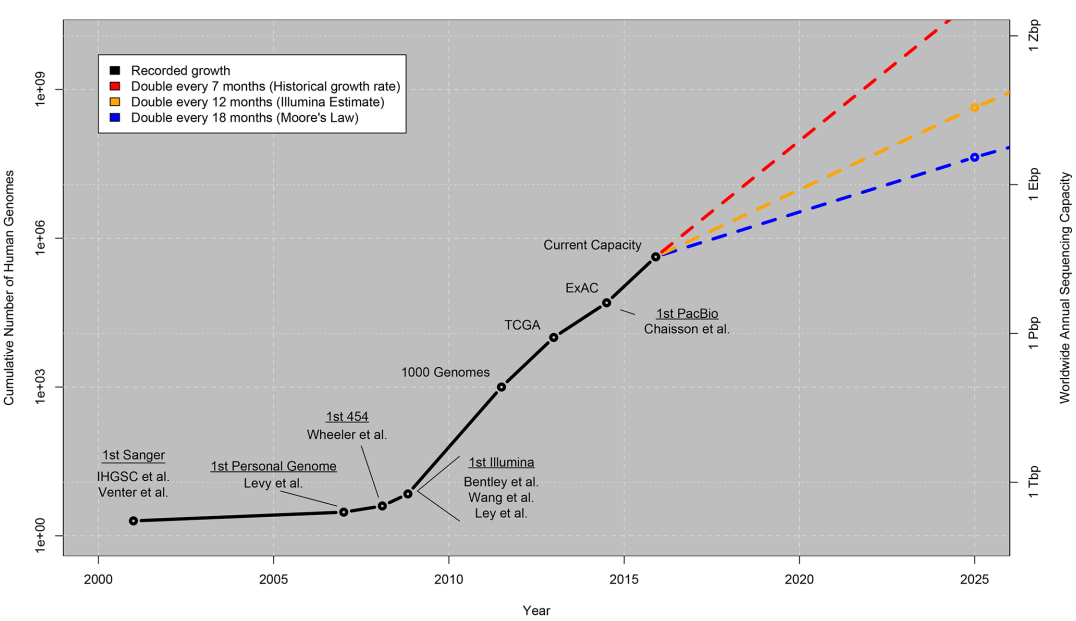
\includegraphics[scale=0.5]{resources/images/Introduction/genomics_growth.png}
\caption{Growth of DNA sequencing \cite{10.1371/journal.pbio.1002195}}
\label{fig:intro_genomics_growth}
\end{figure}

It is clear by now that these volumes need a paradigm shift
from the traditional way we store and analyze data. It is not possible
anymore to store them in a single machine. We need to employ a
distributed system to harness the power of those data and extract
valuable results within a reasonal time frame. On top of that we have
to take under consideration that hardware will fail for various
reasons. A minimum requirement would be not to lose our data, so we
should keep them in several replicas. Going one step further, we would
like our analyzing jobs to continue running even though one machine failed. These
jobs usually take hours to complete, so re-running them is not the
best approach.


%% Longer problem statement
%% General introduction to the area
\section{Problem description}
\label{sec:problem_description}
As it is already mentioned, datasets now days are in the order of
petabytes and exabytes. Distributed file systems like GFS
\cite{Ghemawat:2003:GFS:1165389.945450}, 
GlusterFS \cite{glusterfs}, HDFS \cite{Shvachko:2010:HDF:1913798.1914427} etc come to extend
the traditional file systems located in a single machine. Storing the
datasets is one half of the problem though. The second part is
managing the computational resources on a cluster. A cluster consists
of several physical machines, sometimes thousands of them, and each
machine has numerous CPUs and RAM modules. Users of the cluster issue
their jobs with certain CPU and RAM requirements, as well as the files
which they want to access. On a very high level abstraction there is
an entity which has knowledge of the available resources and should
schedule the jobs accordingly. The view of the cluster from the
\emph{scheduler} perspective is updated frequently with the new
cluster utilization.

This project is a work on Hops \cite{hops} platform
and more specifically on Hops-YARN, which is a modified version of
Apache Hadoop YARN \cite{Vavilapalli:2013:AHY:2523616.2523633}. In YARN the
entity which is responsible for keeping an updated version of the
cluster utilization and scheduling tasks is the \emph{Resource
Manager} (RM). The view of RM regarding the available resources on the
cluster is updated frequently (by default 1 second) by a heartbeating
mechanism. On each machine of the cluster there is the \emph{Node
Manager} (NM) which periodically sends updates for the machine
usage. Users issue their application requests to the RM which then
allocates a container to create the \emph{Application Master}
(AM). The AM service is working independently and is responsible to
keep track of the application health and any further resource
requests. AM periodically heartbeats the RM (by default 1 second)
stating its health, the application progress or any resource
increase/decrease.

An aware reader should have already noticed that RM is a crucial part
of the Hadoop platform for managing resources. Not only it is vital
for the progress of the system but also it can become a
bottleneck and a single point of failure. Until recently, Spotify was
provisioning a cluster of 1300
Hadoop nodes \footnote{http://conferences.oreilly.com/strata/big-data-conference-ca-2015/public/schedule/detail/38595}. Every single node has to heartbeat the RM every
second. On top of that for every single application launched, the AM
service should also heartbeat the RM. This produces a considerable
amount of load on the RM side which has to handle all those heartbeats
and also make scheduling decisions.

In Hops in order to improve performance and HA of the RM we have introduced an
in-memory distributed MySQL database which stores all the necessary
metadata. One great feature of Hops-YARN is that the
\emph{ResourceTrackerService} (RT) of the RM is distributed into multiple
nodes in the cluster. That service is responsible for receiving and handling
heartbeats from the NMs. That way each instance handles only a portion of the total NM
heartbeats. The updated metadata are then stored into the database and
are streamed to the RM to update its view of the cluster. By load
balancing the ResourceTrackerService we have increased the performance
of the system while decreasing the load of the master RM which can
perform the rest of the operations without the load of handling every
single heartbeat.

Another equally important feature of Hops-YARN is that RM stores
every event received and any scheduling decision into the MySQL
cluster. That makes our solution highly available with minimum
failover period. When a RM instance fails it re-builds the view of the
cluster by reading the latest state from the database. More details on
the architecture of both YARN and Hops-YARN will be given in Chapter
\ref{chap:background} and \ref{chap:implementation}.

\section{Problem statement}
\label{sec:problem_statement}
Even with high
throughput, low latency network between the RM/RT and the database, it
still takes more time than in-memory operations. Especially in cases
where RM operations need more than one round-trip to the database, the
difference in performance is noticeable.

A great advantage of using a relational database is the support of
foreign key constraints. The information that we store is semantically
related. In a SQL schema that is directly translated to foreign key
constraints. A trivial example is information regarding the containers
running on node and information regarding the node itself. Clearly, we
should never run into a situation where we try to persist a container
running on a node without having information about the node at
all. Moreover, foreign key constraints work the other way around. By
removing the information about a node from the database we want the
information about running containers on that node to be purged
too. Such constraints, although they seem tempting to use, pose a
great performance degradation as we will show later in this thesis. Particularly when we aim for millions
of operations per second, the use of foreign key constraints should be
limited and very well designed.

The transaction state manager of Hops should try to commit
various states in parallel as much as possible but on the other hand
ensure the order of two colliding states. For example there should
never be the case where two states change information about the same
node in the cluster and yet be committed in parallel. Similarly, two
states that change information in the database about different
entities should be committed in parallel.

The distributed MySQL cluster database is a central building block in our
architecture. A slow commit and process time will result in less events being
streamed and handled by the RM, directly affecting the cluster
utilization and the view of the cluster from the RM perspective.
A slow commit time will decrease the
rate of handled events while increase the rate of queued events that
are waiting to be handled. Our goal is to be able to scale up to 10000 NMs
with multiple RTs. With the current mechanism this is not possible due
to delays both in the transaction manager mechanism and in the commit
time.

\section{Goals, Benefits, Ethics and Sustainability}
\label{sec:goals_ethics}
This is going to be my goals, benefits, ethics and sustainability section...

\section{Structure of this thesis}
\label{sec:thesis_structure}
\section{Structure of this thesis}
\label{sec:thesis_structure}
This is the structure of this thesis

\chapter{Background}
\label{chap:background}
This chapter will give the reader the necessary background knowledge
in order for this work to be understandable. First, it will go through
Apache Hadoop, a distributed storage and processing framework. We will
give some brief introduction to Hadoop file system (HDFS), then we
will dive into the
resource manager (YARN) and in what way HopsYarn extend the Apache
YARN project. Later we will introduce a distributed, highly-available,
highly-redundant relational database, MySQL Cluster (NDB) and finally
we will give some insights on the different types of resource managing
systems.

In Figure \ref{fig:back_hpc_arch_overview} we can see a high level
overview of the architecture in HPC. Storage nodes are machines with very high disk capacity and bare
minimum processing power. Their main usage is to store data that are
going to be processed and analyzed in the future. The second building
block of the architecture is the Computing nodes. These machines have
no storage capabilities but they are equiped with the state of the art
processing units and a lot of RAM. Those modules communicate most
probably with a high throughput, low latency network. The most common
industry standard for interconnecting nodes in HPC is InfiniBand
\cite{infiniband} that it can
reach 30 Gb/s in each direction and sub-microsecond latency. Users
issue their jobs to the Head node which is responsible for transfering
the requested datasets from the Storage nodes to the Computing nodes,
monitor the tasks and finally return the result to the end user.

\begin{figure}
\centering
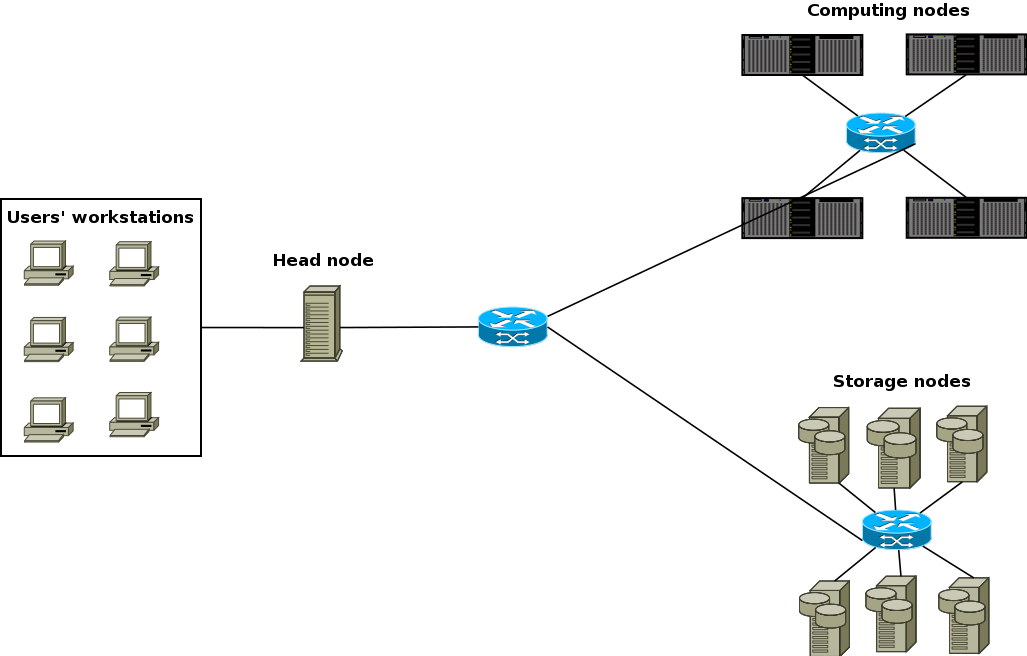
\includegraphics[scale=0.35]{resources/images/Background/hpc_arch_overview.png}
\label{fig:back_hpc_arch_overview}
\caption{HPC high level architecture}
\end{figure}

In 2003 Google published a paper describing GoogleFS (GFS)
\cite{Ghemawat:2003:GFS:1165389.945450}, a proprietary distributed
file system. It was designed to run on large clusters of commodity
hardware, that are doomed to fail at some time. That was the main
motivation that drove GFS to be fault-tolerant and
highly-available. Apache HDFS is the open-source implementation of GFS
and it will be analyzed in Section \ref{ssec:hdfs}. In 2004 Google
published MapReduce \cite{Dean:2004:MSD:1251254.1251264}, a breakthrough programming model which exploited the locality
awareness of GFS and changed the way we process very big
datasets. MapReduce was later implemented for Hadoop and paved the way
for YARN, the current resource manager and scheduler 
which will be analyzed in Section \ref{ssec:yarn}.


\section{Hadoop}
\label{sec:hadoop}
Apache Hadoop is an open-source framework for distributed storage of
large datasets and processing across clusters of computers. It was
created in 2006 after the release of GFS
\cite{Ghemawat:2003:GFS:1165389.945450} and MapReduce
\cite{Dean:2004:MSD:1251254.1251264} papers from Google. The core part
of Hadoop comprises of its distributed file system -- HDFS, and the
job scheduling, resource management framework -- YARN.

The attribute that makes the biggest difference in Hadoop and similar
projects is that of data locality awareness. In contrast to the HPC
architecture, we do not distinguish anymore between processing and
storage nodes. All nodes in a cluster perform both roles. Datasets are
split into blocks of data. To provide fault tolerance each block is
replicated in several nodes in the cluster. Moreover, there is a
central authority which keeps track of the nodes each block is stored.

With that feature in mind, we do not move datasets anymore to the
computing nodes but the executable of our job to the nodes where our
data reside. When the processing of the individual blocks is done, we
gather the result. That is a great paradigm shift from the traditional way
of processing big datasets. A high level overview of the Hadoop
architecture is depicted in Figure
\ref{fig:hadoop_arch_overview}. Datasets are split into blocks and
are stored in the nodes of cluster, both the original and the
replicas. When a user submits a job, the workflow manager will copy
the job to the appropriate nodes, which in parallel will execute
it. Finally, the workflow manager will gather the individual results,
aggregate them and return the final result to the client.

\begin{figure}
\centering
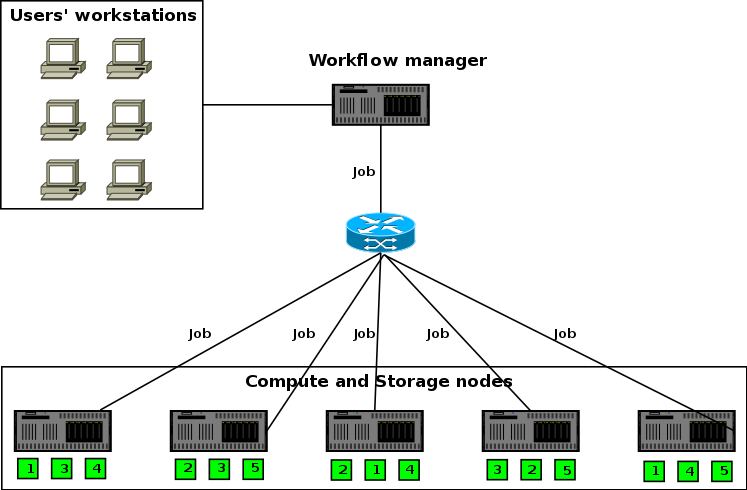
\includegraphics[scale=0.5]{resources/images/Background/hadoop_arch_overview.png}
\label{fig:hadoop_arch_overview}
\caption{Hadoop high level architecture}
\end{figure}

\section{HDFS}
\label{sec:hdfs}
As this project is focused on the resource management framework, I will
not give a detailed description of the Hadoop Distributed File
System. Yet, I will go through some basic concepts that will make the
reader understand better the overall architecture of Hadoop.

HDFS is the distributed file system of Hadoop platform. It is designed
with the assumption that hardware failure is the norm and not an
exception making it highly fault-tolerant. Also, it is designed to run
on commodity, heterogeneous, low-cost hardware making the setup and provisioning of
a cluster cheaper than in HPC. HDFS has two main entities, the NameNode
(NN) and the DataNode (DN) and its architecture is depicted in Figure
\ref{fig:hadoop_hdfs}.

\begin{figure}
\centering
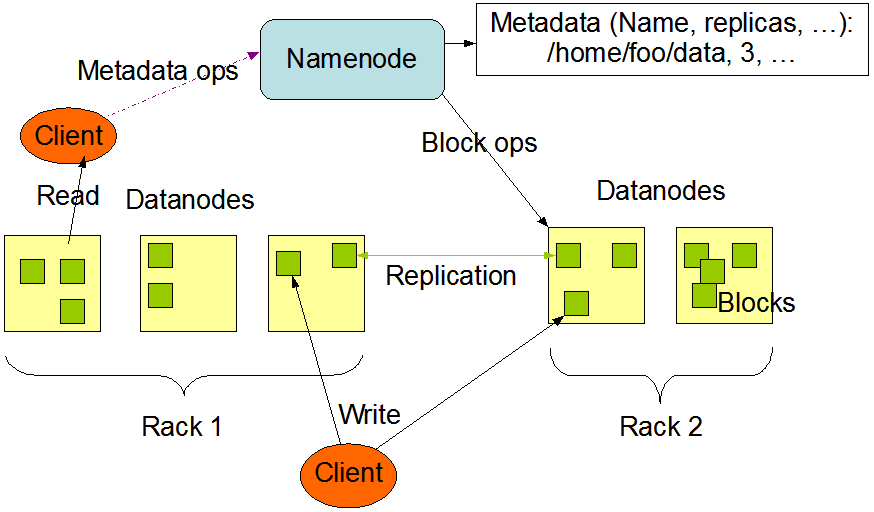
\includegraphics[scale=0.5]{resources/images/Background/hdfs_arch.png}
\caption{HDFS architecture \cite{hdfs}}
\label{fig:hadoop_hdfs}
\end{figure}

\subsection{NameNode}
\label{ssec:nn}

An HDFS cluster consists of a single active NN that is responsible for the
file system metadata, the blocks replication and the health
status of the DNs.

HDFS exposes to a user a file system similar to POSIX, in terms that
the structure is hierarchical, there are the same file permissions 
and a subset of POSIX operations. A user through the NN can open,
close, read, delete a file as in any file system. The NN uses a transaction
log, the \emph{EditLog}, that persists to the local file system any
operation that is done to the HDFS namespace. For example if a file is
renamed then a record is added to the EditLog, or if the replication
factor for a file is changed.

As HDFS was designed to run on commodity
hardware it should be able to handle machine failures. Internally, a
file is split in a number of blocks. Typically each block is 128 MB,
except from the last one and are stored
in the DNs. HDFS replicates the blocks to other machines--DNs
according to a configurable replication factor and replication policy.
If the DN that holds a specific block has crashed, then that block is read from
another replica in another DN.
The NN keeps a file in its local file system with the entire namespace
and the mapping of blocks to DNs, called \emph{FsImage}. Upon
recovery, the NN reads the FsImage and applies any operation that is
logged in the EditLog. That way it can recover from a scheduled
maintenance reboot or from a crash.

The NN periodically receives heartbeats from the DNs that have dual
purpose. The first one is to maintain a health status for the DNs. If
the NN misses a heartbeat from a DN, then it marks that DN as
dead. From that point no blocks will be further assigned to that DN
and NN will start migrating all the blocks that reside in that DN to
others. The second reason of receiving heartbeats is to maintain an
updated view of the \emph{BlockMap}, the mapping of blocks to
DNs. When a DN sends a heartbeat to the NN, it piggybacks a list with
the blocks that it currently stores. That way, the BlockMap in the NN
is kept up-to-date with the blocks that are stored in every DN.

\subsection{DataNode}
\label{ssec:dn}

The DN is the slave entity in the HDFS master/slave architecture as depicted in
Figure \ref{fig:hadoop_hdfs} and the actual storage of blocks. Upon a
client request to store a file in HDFS, the NN instructs it (the
client) which DNs to contact to store the individual file block. The
same procedure is followed when a client requests to read a file. The
NN returns a list with DNs that store the blocks forming the whole
file. The client then contacts each and every DN, fetching the
corresponding blocks.

A DN periodically heartbeats to NN. As I have explained in Section
\ref{ssec:nn}, the heartbeat contains a list of blocks, that the DN
issued the heartbeat stores, so that the NN maintains a map of file
blocks and DataNodes. Also, the heartbeat signifies that the DN is
alive and can be used for storage and retrieval of blocks. Heartbeats
also carry information regarding the status of the DN such as total
storage capacity, storage in use etc. These metrics are taken
consideration by the NN when assigning blocks to DN.

The DataNode also perform various operations as instructed by the
NN. These instructions are sent to the DN via the heartbeat
mechanism as a reply to the heartbeat sent by the DN. Such operations
might be creation, deletion or replication of a block. The block
replication is done according to the replication strategy. A common
strategy for placing replicas with a replication factor of three, is
to place the first replica in the same node as the client runs, the
second in another node in a different rack (off-rack) and the third
one in the same rack as the second but in a different node. Adjusting
the replication factor and the replication policy can greatly affect
the write and read performance of the HDFS cluster and should be
carefully tweaked.


\section{Data computation and Resource management}
\label{sec:resource_mgm}
Something general about MapReduce and YARN resource management

\subsection{MapReduce}
\label{ssec:mapreduce}
After the world wide web explosion at the ending of 1990's, Google has
emerged as one of the most significant web searching companies.
The novelty of Google was PageRank \cite{ilprints361}, an
algorithm counting the number of outgoing links of a webpage to determine its
importance. In order to apply the PageRank algorithm and form the
Google search results, first the webpage has to be scraped and
indexed. As of 2004 the raw size of the documents that had been
collected was more than 20 terabytes
\cite{Dean:2004:MSD:1251254.1251264}. Although the engineers at Google
have distributed and parallelized the algorithm, there were more tasks
that other teams have parallelized in a different way making it
difficult to maintain such a diverse codebase. That led them in 2004
to publish a paper about MapReduce, a generic framework to write distributed
applications that hide all the complexity of fault-tolerance, locality
awareness, load balancing etc.

MapReduce programming model borrows two very common functions from
functional programming, \emph{Map} and \emph{Reduce}. The \emph{Map}
function takes as input key/value pairs and produces as output a set
of key/value pairs as well. The \emph{Map} function is written by the
user and varies depending on the use case.

The \emph{Reduce} function, takes as input the
intermediate key/value pairs produced by \emph{Map} and merge them
together producing a smaller set of values. The \emph{Reduce} function
and the way it will merge the intermediate pairs is also provided by
the user.

A trivial example of the MapReduce programming model is that of
counting the occurrences of words in a text. The \emph{Map} function
takes as input a list of all the words in the text and emits a tuple
in the form \texttt{(word,1)}, where \texttt{word} is every word
parsed. The result of the \emph{Map} function is passed to the
\emph{Reduce} function which adds the value of the tuples with the
same key, in that case is the word. The result will be a list of
tuples where the key is all the words parsed from the text and the
value would be the occurrences of the word in the text.

Google provided a framework which took advantage of the locality
awareness of the already existing GFS and the MapReduce programming
paradigm. The execution overview of MapReduce is depicted in Figure
\ref{fig:mapreduce_execution_overview}. We can identify two entities
in MapReduce architecture, the \emph{Master} and the \emph{Workers}.

\begin{figure}
\centering
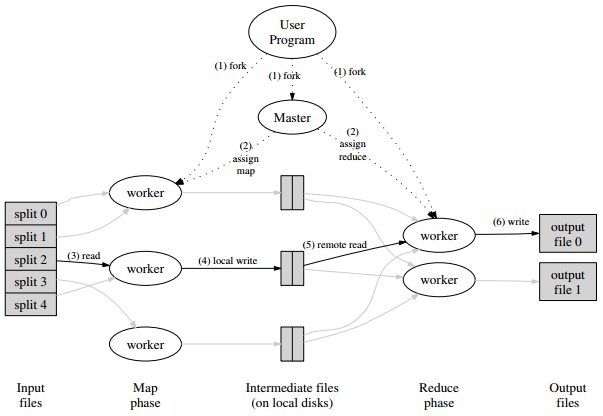
\includegraphics[scale=0.8]{resources/images/Background/mapreduce_exec_overview.png}
\label{fig:mapreduce_execution_overview}
\caption{MapReduce execution overview \cite{Dean:2004:MSD:1251254.1251264}}
\end{figure}

The \emph{Master} has the role of the coordinator that pushes the jobs
to the worker machines. It keeps track of the status of jobs in the
workers, informs other workers for the intermediate files produced
during the Map phase and pings the workers to verify their liveness.

The \emph{Workers} reside at the same physical hardware as the GFS
nodes to take advantage of the data locality. They are divided into
\emph{mappers}, which execute the Map function and \emph{reducers},
which perform the reduce phase as instructed. Workers are
pre-configured with available map or reduce slots depending on their
CPU or RAM.

At the very beginning, a user submits a job to Master. Master forks
the submitted job and is responsible to schedule the forks on workers
that $(a)$ have available map/reduce slots and $(b)$ have the
requested datasets stored locally. Upon the scheduling is done, the
Map phase begins in the mappers. They read the datasets from the local
hard drive and perform the Map function. Master periodically pings the
mappers to get informed about the status of the job and the health of
the node itself. When a mapper node completes its task, it writes the
intermediate key/value pairs to the local file system and informs the
Master node. The Master node in turn, notifies the reducer nodes that
an intermediate result is available at a specific node, where the
latter reads it (the result) remotely and perform the reduce
function. Finally, when all the reducers have completed the Reduce
phase, the Master notifies the user program.

\subsubsection{MapReduce Fault Tolerance}
Primary concern of the engineers was the fact
that machines will eventually fail. MapReduce will run on a cluster of
thousands of machines so the probability of a failed machine would be
higher. For that reason they equipped MapReduce with a heartbeating
mechanism in order to be able to handle such situations.
The Master periodically pings the workers. The workers should respond back
within a predefined timeout before they are declared dead. When a node
that performs the Map phase is declared dead, then the job that was
running at that node is set to \emph{idle} and is rescheduled on
another node. Similarly, when a map job has finished, since the
intermediate result is written to the local hard drive, the job has to
be rescheduled in a different machine. When a reducer node has failed
and the job is still in \emph{running} state, then it is set back in
\emph{idle} state and assigned to another node. In case of a completed
Reduce phase, the result is stored in the global file system, GFS in
that case. So, even with a failed reducer machine, the result will
still be available and the job should not be rescheduled.

While a Worker failure does not greatly affect the MapReduce job, it
is not the same case with a Master failure. If a machine that is a
Master node fails, then the whole MapReduce job is canceled and the
client is informed so that it can retry later on. ``However, given
that there is only a single master, its failure is unlikely;''
\cite{Dean:2004:MSD:1251254.1251264}.

\subsubsection{Limitations}
MapReduce facilitated engineers to ``easily'' write parallel data
processing applications by hiding all the complexity of a distributed
system. It provided some sort of fault tolerance and it was generic
enough to fit in various domains.

MapReduce and Hadoop over the years has become the industry standard
for processing and storing big volumes of data. After some period of
heavy usage it became clear that, although the platform itself suited
the needs for distributed, reliable storage and cluster management,
there were some limitations that had to be addressed. The two key
shortcomings were regarding the tight coupling of a programming model
with the resource management infrastructure and the centralized
handling of jobs \cite{Vavilapalli:2013:AHY:2523616.2523633, 6680946}.

A user who wanted to write an application for MapReduce framework,
all it had to do was to provide implementation for the two
first-order functions \emph{Map} and \emph{Reduce}. This static
map-reduce pipeline is very limiting though, as every job should have exactly one
Map function followed by an optional Reduce function. That workflow is
not suitable for large scale computations, such as machine learning
programs that require multiple iterations over a dataset. That means
that multiple individual MapReduce jobs had to be scheduled while the
frequent write of data in disk or in a distributed file system would
impose a considerable latency. A common pattern/misuse
\cite{Vavilapalli:2013:AHY:2523616.2523633} was to submit jobs with a
map phase only that spawned alternative frameworks or even web
servers. The scheduler had no semantics about the job except that they
were map jobs with a consequence in the cluster utilization, creating
deadlocks and a general instability to the system. The second drawback
of MapReduce and Hadoop 1.x was the centralized job handling and
monitoring of their flow. The Master or the \emph{JobTracker} should
monitor every single job, receiving liveness heartbeats, resource
requests etc. The is a heavy workload for a single machine that drove
to major scalability issues.

These two crucial limitations of MapReduce led to a total re-design of
Hadoop. Since Hadoop 2.0 there is a resource management module, YARN --
\emph{Yet Another Resource Negotiator} which will be analyzed in
section \ref{ssec:yarn} and MapReduce is just another application
running on a cluster of physical machines.

\subsection{YARN}
\label{ssec:yarn}
Considering the limitations outlined in section
\ref{sssec:mapreduce_limitations}, Vinod Kumar Vavilapalli et
al. presented YARN \cite{Vavilapalli:2013:AHY:2523616.2523633} the new
resource management layer that was adopted in Hadoop 2.0. The new
Hadoop stack now is depicted in Figure \ref{fig:yarn_hadoop1_hadoop2_arch} where YARN is the
cluster resource management module and MapReduce is one out of plenty
applications running on top of YARN. This architectural transformation
paved the way for a wide variety of frameworks like
Apache Spark \cite{apache_spark}, Apache Flink \cite{apache_flink},
Apache Pig \cite{apache_pig}, etc to run on the
Hadoop platform like any other YARN application.

\begin{figure}
\centering
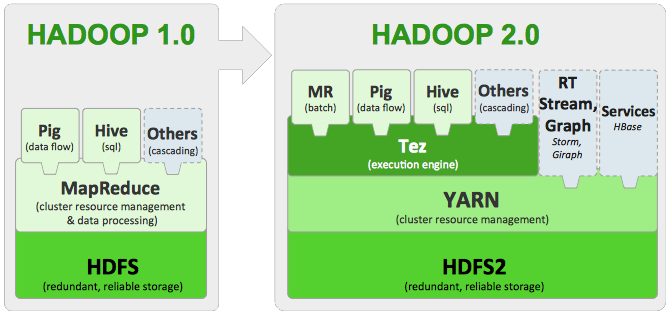
\includegraphics[scale=0.6]{resources/images/Background/hadoop1_hadoop2_arch.png}
\label{fig:yarn_hadoop1_hadoop2_arch}
\caption{Hadoop 2.0 stack \cite{hortonworks_hadoop_stack}}
\end{figure}

The new architecture of Hadoop 2.x separates the resource management
functions from the programming model. It delegates the
intra-application communication and the tracking of the execution flow
to per-job components. That unlocks great performance improvements,
improves scalability and enables a wide variety of frameworks to share
the cluster resources in a very gentle way.

YARN uses three main components to provide a scalable and fault
tolerant resource management platform. The first component is the
\emph{ResourceManager} (RM), a per-cluster daemon that tracks resource
usage and node liveness and schedules jobs on the cluster. The second
component is a per-node \emph{NodeManager} (NM) which is responsible
for monitoring resource availability on the specific node, reporting
faults to RM and managing container life-cycle. Finally, there is the
\emph{ApplicationMaster} (AM) which coordinates the logical plan of a
single job, manages the physical resources offered by the RM and
tracks the execution of the job. A high level overview of YARN
architecture is described in Figure \ref{fig:yarn_arch_overview}. RM
has a global view of the cluster and provides the scheduling
functionality, while the per-job AM manages the dynamic resource
requests and the workflow of the tasks. Containers that are allocated
by the RM are locally managed by the NM in each node in the cluster.

\begin{figure}
\centering
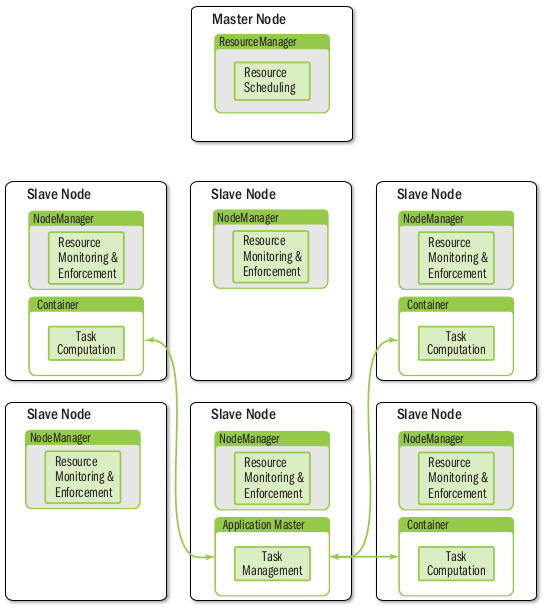
\includegraphics[scale=0.5]{resources/images/Background/yarn_arch_overview.png}
\label{fig:yarn_arch_overview}
\caption{YARN architecture overview \cite{Murthy:2014:AHY:2636998}}
\end{figure}

\subsubsection{ResourceManager}
\label{sssec:rm}
In YARN the RM acts as the central authority for allocating resources
in the cluster. It works closely with the per-node NodeManager getting
an updated view of the cluster by the heartbeats received. The RM
itself allocates generic resources in the cluster in the form of
\emph{containers} that have specific CPU and RAM requirements. Those
resource requests are piggybacked in the heartbeats issued by every AM.
As RM is completely unaware about the job execution plan,
it is up to the AM to make local optimizations and assign the
resources accordingly. RM internally consists of several modules but
the three most important are the \emph{ApplicationMasterService}, the
\emph{ResourceTrackerService} and the \emph{Yarn Scheduler} as shown
in Figure \ref{fig:yarn_RM_components}.

\begin{figure}
\centering
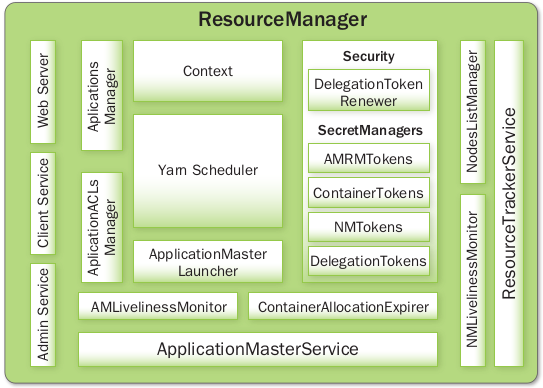
\includegraphics[scale=0.6]{resources/images/Background/RM_components.png}
\label{fig:yarn_RM_components}
\caption{ResourceManager components \cite{Murthy:2014:AHY:2636998}}
\end{figure}

The \emph{ApplicationMasterService} is responsible for receiving and
handling heartbeats from the AMs that are launched in the
cluster. Heartbeats are designed to be as compact as possible, still
not excluding any vital information. For that reason, Google Protocol
Buffers \cite{proto_buf} are used for every communication among YARN
components. Protocol Buffers is a language-neutral, platform-neutral
mechanism for efficiently serializing data. The heartbeat mechanism
serves both as a scalable way for the RM and AM to communicate, but
also for the RM to track the liveness of AMs. \emph{ResourceRequests}
contain information such as the resources per container in terms of
virtual cores and memory, the number of containers, locality
preferences and priority of requests. The scheduler then tracks,
updates and satisfies these requests with available resources in the
cluster. The RM builds the view of the cluster with the available
resources from the information it receives from the NMs. The scheduler
tries to match the locality constraints as much as possible and
responds back to AM with the allocated containers along with
credentials that grant access to them. The RM also keeps track of the
AM health through the heartbeats received. The component that handle
the liveness property of every AM is the \emph{AMLivenessMonitor}. In
case of a missed heartbeat, that particular AM is deemed dead and
is expired by the RM. All the containers that were allocated for
that AM are marked as dead and the RM reschedules the same application
(ApplicationMaster) on a new container.

As I have previously mentioned, the RM builds its view of the cluster
by the information that NMs send to it. The
\emph{ResourceTrackerService} component is responsible for handling such RPCs
and forwarding them to the appropriate modules. Before a new node in the
cluster is able to execute YARN jobs, it should first register itself
with the RM through the ResourceTrackerService and exchange some
security tokens. A heartbeat mechanism is also used in this place to
ensure the liveness of NMs and to receive updated information about
the available resources in the physical machine. The newly received
information about the available resources on that node is forwarded to the YARN
scheduler so it can make scheduling decisions. Also, a received
heartbeat is forwarded to the \emph{NMLivelinessMonitor} module which
keeps track of the health of NMs. If RM has not received any heartbeat
from a NM after a configurable timeout, then it is deemed dead and is
expired. All the containers that were currently running on that node
are also marked as dead and an event is sent to the scheduling module
not to schedule any job on that node. When the node restarts, it
registers again with the RM and it makes itself available for
scheduling again.

At the core of RM is the \emph{YarnScheduler} that is responsible of
making scheduling decisions based on the available resources on the
cluster and the resource requests issued by the AMs. Currently the
resource requirements of an AM are limited to the number of virtual
cores and to the amount of memory a container should
have. YarnScheduler is a pluggable module and at the time of writing
there are three different options. The first and original option is
the \emph{FIFO Scheduler} where jobs are served in a simple
first-in-first-out order with no sense of priorities. The second
scheduling policy is the \emph{Capacity Scheduler}
\cite{capacity_scheduler} developed by Yahoo! Capacity Scheduler
is primarily built for large clusters with resources that are shared
among different units in the same organization. There are different
queues serving jobs for various units while guaranteeing some minimum
capacity for each queue. Any excess capacity can be temporarily
allocated to other queues and a job with high priority will be executed
before any other job with lower priority. If a job cannot be scheduled
in its respective queue due to lack of resources and that queue is
below its fair share, then jobs in other queues can be preempted. Last
but not least is the \emph{Fair Scheduler} \cite{fair_scheduler}
developed by Facebook. In Fair Scheduler every application belongs to
a queue, by default the ``default'' queue. The basic idea is that
containers are allocated to the application with the fewer resources
assigned within the queue, providing a uniform distribution of the
available cluster resources in the long run. There can be multiple
queue with support for priorities, minimum and maximum shares and FIFO
ordering within the queue. Similar to Capacity Scheduler, Fair Scheduler
also has support for preemption of containers that are already
assigned. Currently the default scheduler for Hadoop is the Capacity Scheduler.

\subsubsection{ApplicationMaster}
\label{sssec:am}
Upon a successful submission of an application to RM, the latter
creates a special container in a node called
\emph{ApplicationMaster}. AM is a per-application process that
coordinates the execution plan of the application, negotiates
resources with the RM and monitors the assigned containers. AM
periodically heartbeats RM, default value is 10 minutes, to prove it
is alive and to dynamically request more resources or release
some. When AM is launched, it will compute the necessary requirements
and locality preferences, encode them and through the heartbeat
mechanism send them to RM. RM depending on the scheduling decisions it
has made it might respond back with any empty response or with
\emph{container leases} on different nodes. AM will contact the
respective NodeManagers, present them the leases and the NM will
create the containers. Afterwards, it (AM) is responsible to monitor the liveness
of the containers or implement any recovery functions. An overview of
the workflow explained above is illustrated in Figure \ref{fig:yarn_am_rm_interaction}.

\begin{figure}
\centering
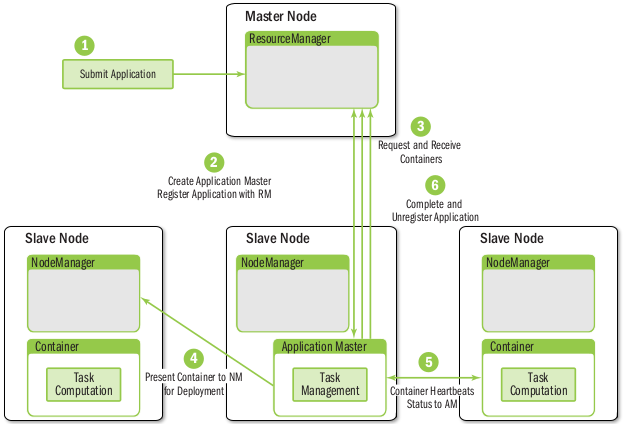
\includegraphics[scale=0.6]{resources/images/Background/AM_RM_interaction.png}
\label{fig:yarn_am_rm_interaction}
\caption{ApplicationMaster interaction \cite{Murthy:2014:AHY:2636998}}
\end{figure}

Since a key requirement for YARN was to decouple the programming model
from the resource management, AM is not tightly connected to YARN.
Writing an ApplicationMaster process is not an easy task but Hadoop
offers some APIs to avoid the complexity of low-level protocols.
Users can write their own ApplicationMaster
process fitting particular needs of making local optimizations with
the containers allocated by the RM, monitoring the containers,
define the recovery procedures when a container dies or capture the
exit status of a finished task. That opened the road for a plethora
of applications to run on Hadoop such as Apache Spark
\cite{apache_spark}, Apache Flink \cite{apache_flink}, Apache Hadoop
MapReduce \cite{apache_hadoop} etc.

\subsubsection{NodeManager}
\label{sssec:nm}
The \emph{NodeManager} is the ``worker'' daemon that runs on every
physical node of a Hadoop cluster. It is responsible for monitoring
the health of the physical hardware, authenticating the container
leases, preparing, monitoring and tearing down the container and
providing a set of services to the application.

When a node joins a cluster, the NM should register with the
RM. It will present the total amount of virtual cores and memory
available in this machine, some security tokens required to
authenticate the container leases, some communication ports etc. From
that point NM should periodically heartbeat the RM, default value is 1
second, proving that is still alive and keeping the RM up-to-date with
its status. NM regularly runs some monitoring scripts for the
health of the machine and the status is sent to RM. As a response it
might get back a list of container leases or some instructions such as
node decommission because of unhealthy node or to kill some
containers. In case of a missed heartbeat, the RM declares the NM as
dead, excludes that node from its pool of resources and informs all
running AMs about the failed NM. AM is responsible to react to such a
failure and possibly ask resources from RM to redo the work done in
the failed node.

Each container in YARN comes along with a \emph{container launch
  context} (CLC). The CLC contains information specific to the
application that is about to run such as environment variables,
dependencies stored in HDFS or on-line, security tokens, commands that
actually spawn the application etc. Once the NM has validated the
container lease with the security tokens provided, it should
initialize the container by fetching the requested dependencies,
setting the variables and of course run the commands specified by the
CLC. At the end of the container life-cycle or if the container dies
or if RM instructs NM to kill a container, NM should garbage collect
any dependency fetched during initialization and not used any
longer by other containers in that node. For the whole duration of a
container's life-cycle, NM monitors its utilization. If a container's
usage exceeds its assigned, then the NM signals the container to be
killed so that it does not disrupt the work of other containers
sharing the same physical machine. 

Finally, NM provides some services to the containers such as log
aggregation that will upload anything written to \texttt{stdout} or \texttt{stderr} to
HDFS when the application finishes. NM also provides a set of
auxiliary, pluggable services that are used by some applications. For
example, in MapReduce the intermediate output of the Map phase should
not be garbage collected after the container has finished. The
service will flag these data to be persisted even after the container
has gracefully exit.

\subsubsection{YARN fault tolerance \& HA}
\label{sssec:yarn_ha}
So far we have gone through some key points of the resource management
platform of Hadoop. RM is the central authority that makes scheduling
decisions and carries all the burden of monitoring both the AMs and
the NMs. Although from the beginning Hadoop was designed to run on
commodity hardware where machine failures are the norm
\cite{doi:10.2200/S00516ED2V01Y201306CAC024, Dean:2013:TS:2408776.2408794}, a
ResourceManager failure would drove the whole cluster
useless. Moreover, after a RM restart, it had to kill all the
containers running on the cluster including the ApplicationMasters and
launch new instances of them. Since RM is not responsible for the
recovery of the applications AMs had to start over the tasks, unless if
they had some recovery policy. Hadoop 2.4 introduced some kind of recovery mechanism that would
recover some application metadata and re-submit only the non-finished
applications in a way invisible to the user. As of Hadoop 2.6 RM
restart has further improved. The rest of this section will briefly
explain the recovery and HA mechanism of the RM.

To recover from a failure, RM needs to
store some state in a persistent storage. Currently there is support
for three alternatives. The first one is to use the Apache ZooKeeper
\cite{Hunt:2010:ZWC:1855840.1855851}, a service that provides highly reliable
distributed coordination, naming, storing and group membership
services. The second alternative is LevelDB \cite{google_leveldb},
a light-weight key-value store and finally the local file system or
HDFS. The default state store is the file system, local or HDFS, although
if a requirement of our cluster is also HA, then Apache ZooKeeper is
the preferred one. To begin with, RM stores some application metadata to
the persistent storage solution. These metadata include the
application submission context, the final status of the application,
diagnostics of the application and some security related
tokens. Moreover, when the RM restarts it will ask from all the NMs in
the cluster to re-sync and send back information about all the
containers that are currently running. Using that information it can
recover the whole state of the scheduler such as resource requests,
queues' usage etc. That way RM does not need to kill and kick-off again all
the running applications, just instruct the respective AMs to re-sync
with it.

Even with the aforementioned mechanism RM is a single point of
failure. In case of an RM crash, the cluster would be essentially useless until
the RM restarts and recover. This period, depending on the number of
nodes on the cluster, the number of applications running and the
policies to detect a dead machine, might take quite a long time. As of
Hadoop 2.4 there is a High Availability feature for the RM, using an
Active/Standby architecture and a ZooKeeper instance to coordinate
the RM nodes. ZooKeeper
ensures that at any point of time there is only one Active node that
performs all the scheduling decisions and monitoring operations. In case of a crash, a new leader is elected
from the Standby pool and is promoted to Active. The transition from
Standby to Active can be done either manually through the administration
CLI or automatically where ZooKeeper will detect the crashed node and
elect a new leader. The new Active RM will build the current state
from the state stored in ZooKeeper. AMs and NMs will keep contacting
the crashed, previously Active, RM until they realize it is dead. Then
they will contact the next RM in their configuration list until they
hit the currently Active node in a round-robin fashion.

\section{Distributed databases}
\label{sec:distributed_db}
Some stuff about distributed DB and mainly MySQL cluster NDB

\section{HopsYarn}
\label{sec:hopsyarn}
Hops-YARN is a drop-in replacement of Apache Hadoop YARN for the Hops
\cite{hops} platform. From a user's perspective there is no difference
between the two implementations and an Apache YARN application can be
scheduled on Hops-YARN without any modification. Although the
interface is the same, there are some key characteristics that
distinguish the two implementations and can be categorized into
architectural, recovery mechanism and load balancing. In the rest of
the section I will present the differences in every category.

\subsection{Architecture}
\label{ssec:hopsyarn_arch}
In Hops we heavily use a MySQL Cluster that was briefly introduced in
Section \ref{sec:ndb}. We store all kinds of metadata spanning from
Hops-YARN to Hops-HDFS, a new distribution of Apache HDFS, and
HopsWorks, a web-based UI front-end to Hops. The fact that everything
is stored in the database leverages the limited amount of information
that can be stored in the JVM heap of a single machine and opens up
great opportunities of improvement and experimentation.

Apache Hadoop uses ZooKeeper to detect failures and elect a new leader.
Since the MySQL Cluster is already in place storing data, we use a
leader election mechanism proposed by Salman Niazi et
al. \cite{Niazi2015} that uses NewSQL databases in a novel way.
The protocol guarantees a single process acting
as a leader at any point of time with performance comparable to
Apache ZooKeeper. Having the database acting as a persistent storage
and as a leader election mechanism, Hops drops ZooKeeper from its
stack releaving the operations team from the burden of maintaining
one extra service.

\subsection{Fault tolerance \& HA}
\label{ssec:hopsyarn_fault_tol_ha}
In Section \ref{sssec:yarn_ha} I have outlined how Apache Hadoop YARN
deals with RM failures and provides a highly available solution. In
Hops-YARN we follow a different path for storing information for
recovery. In YARN, AMs and NMs communicate with the RM through a
heartbeating mechanism. These heartbeats carry information such as
(de)allocation requests, health status, etc Since the database allows
for millions of transaction per second, we store every single RPC that
the RM receives and delete them when the request is handled. Moreover,
every operation that is done on the scheduler state is reflected on a
modification in the database. The main advantage of this approach over
the approach followed by Apache YARN is in terms of recovery
time. It is much faster to read the complete state of the scheduler from the
distributed in-memory database than asking from every NM to re-sync
and send back a list of all running containers. Particularly when
the cluster size grows in the order of thousands of
machines. Moreover, in case of a crash in Apache YARN, the RM
instructs all the AMs and NMs to re-sync and send again any request
that has been sent but not handled. In Hops-YARN, the RM recovers the
unhandled RPCs from the database and replays them.

In terms of HA the architecture of Hops-YARN is basically the same
with an Active/Standby model for the scheduler, although some
improvements have been made for the Standby nodes described in the
following section.

\subsection{Load balancing}
\label{ssec:hops_yarn_load_balance}
Standby is boring! Except for being boring, having a physical machine
idle for most of the time is a waste of resources. Although RM is a
monolith, its architecture is modular. The components of the RM are illustrated in
Figure \ref{fig:yarn_RM_components}. Hops-YARN follows a very original
approach of distributing the \emph{ResourceTrackerService} among the
StandBy RM nodes. The \emph{ResourceTrackerService} is responsible for
handling the RPCs from the NMs (see Section \ref{sssec:rm}). Assume a
cluster with the moderate size of 5000 nodes and the default value of 1
second for the heartbeat interval. That implies that every second the
RM should handle 5000 RPCs just for keeping track the NM status. In
Hops-YARN, the StandBy RMs also run the
ResourceTrackerService. When NMs register with the RM they are
assigned to the least overloaded \emph{ResourceTracker} (RT) -- StandBy
\emph{ResourceManager}. The information received by each
\emph{ResourceTracker} separately is stored in the
database and through the event API of NDB is streamed to the Active
RM to update its view of the cluster. In that case, NDB serves as a
communication channel between the RT and the RM. With that
architecture the load of tracking 5000 nodes is distributed among all
the RMs in the cluster. An overview of Hops-YARN distributed
ResourceManager is illustrated in Figure \ref{fig:hopsyarn_dist_rm}.

\begin{figure}
\centering
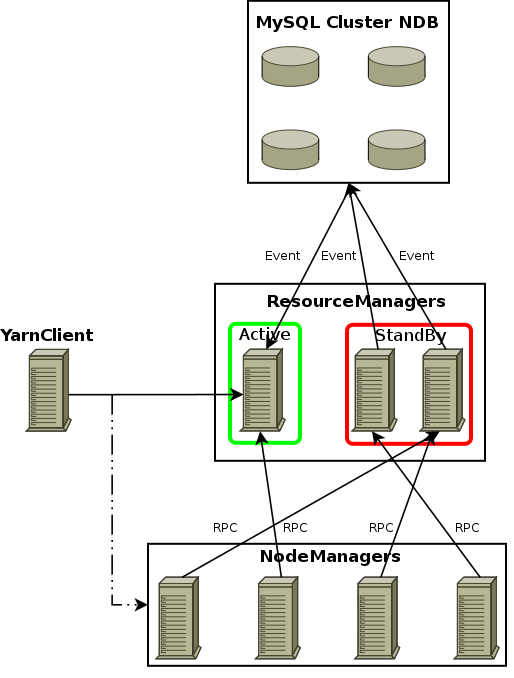
\includegraphics[scale=0.5]{resources/images/Background/hopsyarn_arch_overview.png}
\caption{Hops-YARN distributed RM architecture}
\label{fig:hopsyarn_dist_rm}
\end{figure}

\section{Taxonomy of schedulers}
\label{sec:taxonomy_of_schedulers}
Operating large-scale clusters is expensive both in terms of
investement to buy all the necessary hardware equipment but also in terms of
human resources that will maintain them. The variety in the jobs
running in a big organization poses a great challenge in the
utilization and efficiency of a cluster. There are long-running
production jobs that should ``never'' stop running, short-living
memory intensive batch jobs that analyze massive amount of data,
testing jobs running with the lowest priority and so forth. At the
same time schedulers should be able to scale to tens of thousands of
nodes per cluster and be highly available with minimum downtime. In order
to tackle these issues there has been a lot research regarding cluster
schedulers or datacenter operating systems as they are also
refered. In this section I will present three different architectures
identified in the current literature based on the taxonomy published
in the Omega paper \cite{41684}. An overview of these architectures is
depicted in Figure \ref{fig:sch_tax}.

\begin{figure}
\centering
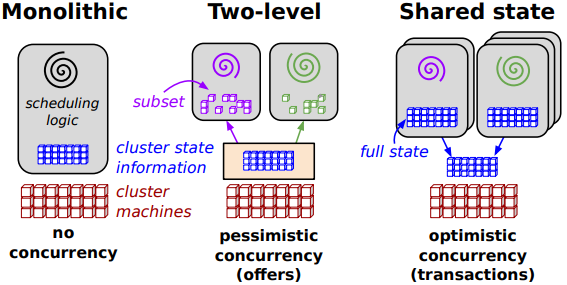
\includegraphics[scale=0.6]{resources/images/Background/schedulers_taxonomy.png}
\label{fig:sch_tax}
\caption{Cluster schedulers architecure \cite{41684}}
\end{figure}

\subsection{Monolithic}
\label{ssec:tax_monolithic}
The first category of schedulers explored is the \emph{monolithic}. In
this architecture there is a single, centralized entity that makes all
the scheduling decisions with no parallelism. A monolithic scheduler
still can facilitate different scheduling policies according to the type
of the workload by providing multiple code paths. Depending on the
type of the job, the execution flow can take different path --
policy. Although, it is tempting to support multiple
scheduling policies, ``it is surprisingly difficult to support a wide
range of policies in a sustainable manner using a single-algorithm
implementation'' \cite{41684}.

Another drawback of monolithic schedulers is the head-of-line
blocking. A small and easy to schedule job might get stack behind a
big and demanding job. This will delay the execution of the former, a
side effect that is not desirable in the enterprize world. Scalability
is another issue that has to be addressed. Since the scheduler runs on
a single instance it can be the bottleneck if the cluster size is big
enough. On the other hand, a monolithic scheduler has a full view of the
cluster and its available resources. For that reason it can make
optimal decisions on the job placement and achieving high utilization
(until it becomes the bottleneck).

A slight variation of a monolithic scheduler is the static
partitioning of the cluster. Each partition will run its own
monolithic scheduler with a separate policy according to the jobs
type. This approach though leads to fragmentation and to sub-optimal
cluster utilization.

A prominent example of a monolithic scheduler is Apache Hadoop YARN
and Hops-YARN. The key characteristic of Hops-YARN is that the state of the
scheduler is stored in the MySQL Cluster which opens the way for
various architectural experimentations resembling shared state schedulers (see
Section \ref{ssec:tax_shared_state}).

\subsection{Two-level}
\label{ssec:tax_two_level}
Two-level

\subsection{Shared state}
\label{ssec:tax_shared_state}
Shared state

\chapter{Method}
\label{chap:method}
%% What are your goals? (What should you be able to do as a result of your solution - which couldn't be done well before you started?)
%%  What you are going to do? Why?
This is going to be the method

\chapter{Analysis}
\label{chap:analysis}
%% How you are going to evaluate what you have done?
%% Analysis of your data and proposed solution
%% Does this meet the goals which you had when you started?
This is going to be the analysis...

\chapter{Conclusions}
\label{chap:conclusion}

\section{Conclusion}
\label{sec:conclusion}
In Hops-YARN, as it is already mentioned, MySQL Cluster NDB is used
both as a communication transport and as a persistent storage for
recovery. At the beginning of the project a thorough profiling of the
execution workflow has been done to identify the bottlenecks of the
system. The first step was to remove the foreign key constraints from
the database schema used by Hops-YARN. In Section
\ref{sec:fk_constraints} is explained how they were replaced by
application logic that performs primary key operations. Section
\ref{sec:tx_aggregation} discusses the evolution of the commit
mechanism which squashes several blocked transaction into a ``big''
one reducing the number of commits in the back-end database
system. Section \ref{sec:gc_service} presents the Garbage Collector
service of Hops-YARN that removes asynchronously old values from the
database. With that solution the commit time dropped more improving
the overall performance of the system. Finally, Section
\ref{sec:dto_caching} explains how the shortcoming of ClusterJ for
creating DTOs was bypassed by having created them ahead of time in a
per session cache.

After a detailed explanation of the solutions proposed, in Chapter
\ref{chap:evaluation} follows the evaluation. Each solution is
evaluated separately by simulating real world traces. In each case key
characteristics are examined and how they have been improved. In
Section \ref{sec:performance_overview} there is an overall performance
overview in terms of cluster utilization and heartbeats processed by
the scheduler. The comparison is made among the version of Hops-YARN
before this project, the final version with all the modification
proposed and the upstream Apache YARN. The figures show that there was
a clear improvement, in both evaluation parameters, when the two
version of Hops-YARN are compared. Finally, as far as the cluster
utilization is concerned, the performance is comparable with Apache
YARN in clusters with thousands of nodes.

\subsection{Goals}
\label{ssec:goals}
In Chapter \ref{chap:introduction} the goals of this project were
set. The primary goals was to improve the cluster utilization and the
number of heartbeats processed by the scheduler. In order to achieve
those goals we have also set some sub-goals. With the solutions proposed
in Chapter \ref{chap:implementation} all the sub-goals were met. In
particular, with the removal of the foreign key constraints and the
DTO caching mechanism the transactional commit time was decreased
dramatically. Some sort of asynchronous API was provided by the
garbage collector service. It is provided only for a small sub-set but
still it made big difference to the performance of the system. The new
aggregation mechanism of the transaction manager of Hops-YARN helped
the blocked transactions to be committed faster which in turn improved the
parallelization of the system. Finally, in each step of the
implementation an evaluation was done to prove the performance impact
and guide us to new bottlenecks.

Since all the sub-goals were met it was expected to achieve the
primary goals. As Chapter \ref{chap:evaluation} indicates the two
primary goals were also accomplished. Both cluster utilization and the
heartbeat ratio was improved.


\subsection{Insights and suggestions for further work}
\label{ssec:insights-and-suggestions}
This is the insights section

\section{Future work}
\label{sec:future-work}
A few things have been left undone due to time limitation and are
discussed in this section for future work.

In most of the cases the evaluation has been done using simulations
measuring among others the cluster utilization while in others the
evaluation has been done using benchmarks. It would be more complete
if in all cases the benchmarks were supported by simulation
results. That way the performance improvements introduced by each step
would be more clear.

Currently we do not have any insight on the content of Transaction
State objects, thus they are treated equally. In real world scenarios,
during the allocation of resources, the Transaction State would carry
more information about allocated containers than when the cluster is
full and no further allocations can be made. A fine-grained inspection
on the content of a TS might improve performance further more. For
example in the commit mechanism, when an Aggregated Transaction State
object is overloading NDB, the transaction will roll-back and the
aggregation policy will enforce a lower limit. If we had any
information on the content of the TS before hand, this situation could
have been avoided.

As it is already mentioned, the Garbage Collector service does not
perform primary key operations. It was a design decision that would
not complicate the mechanism and burden the commit time by committing
more information. It is worth trying to persist all the columns needed
for the primary keys to be reconstructed and measure the
performance. For sure the deletion time would be lower but it
remains to be proven if that will have any impact on the performance
of Hops-YARN in general.

Last but not least, the batching system explained in Section
\ref{ssec:impl_batch_system} should be improved. Changing the number
of RPCs that are batched together did not change the
performance. Every RPC arriving in the ResourceManager among others it
should get the current Transaction State object from the Transaction State
Manager. This operation could take $0.06$ ms. If we consider a cluster
with 10000 NodeManagers heartbeating every second, it is needed 600 ms
just to acquire the object. At the time of writing that was the latest
bottleneck encountered and for sure it is worth for future investigation.

\subsection{What has been left undone?}
\label{ssec:what-has-been-left-undone}
This is what has been left undone


%%\bibliography{report}
%%\bibliographystyle{IEEEtran}
%%\bibliographystyle{unsrturl}
%%\bibliographystyle{unsrtnat}
%%\bibliographystyle{myIEEEtran}

\printbibliography[heading=bibintoc]

\appendix
\chapter{Insensible Approximation}

\backmatter

\end{document}
